\section{Extras}

\subsection{Standardbibliothek}\label{sectionStandardBibliothek}

Mithilfe interner Funktionen soll die Klippe zwischen Sprache und Systemoperationen überbrückt werden.
In der Package \texttt{standardLibrary} werden diese internen Funktionen in Java umgesetzt.

Dabei implementiert jede interne Standardbibliotheksfunktion die Methode \\
\texttt{compute(Object... objects)} aus dem Interface \texttt{InternalFunction}.
Die jeweilige Implementierung wird zusammen mit den geforderten Parametern und einem Funktionsnamen vor dem Start des Interpreters in dessen Environment gepackt.
Wird aus Tabulang die entsprechende interne Funktion wie zum Beispiel \texttt{print(123)} aufgerufen, wird im Interpreter die korrekte Anzahl der Parameter überprüft und mit dem Aufruf der \texttt{compute} Methode die entsprechende interne Funktion ausgeführt.

In Abbildung \ref{fig:standardlib-uml} wird zusätzlich gezeigt, wie die statischen Methoden in \texttt{StandardLibrary} durch alle verfügbaren Funktionsklassen geht, ein Objekt davon erstellt und dieses dem Interpreter hinzufügt.

\begin{figure}[h]
\centering
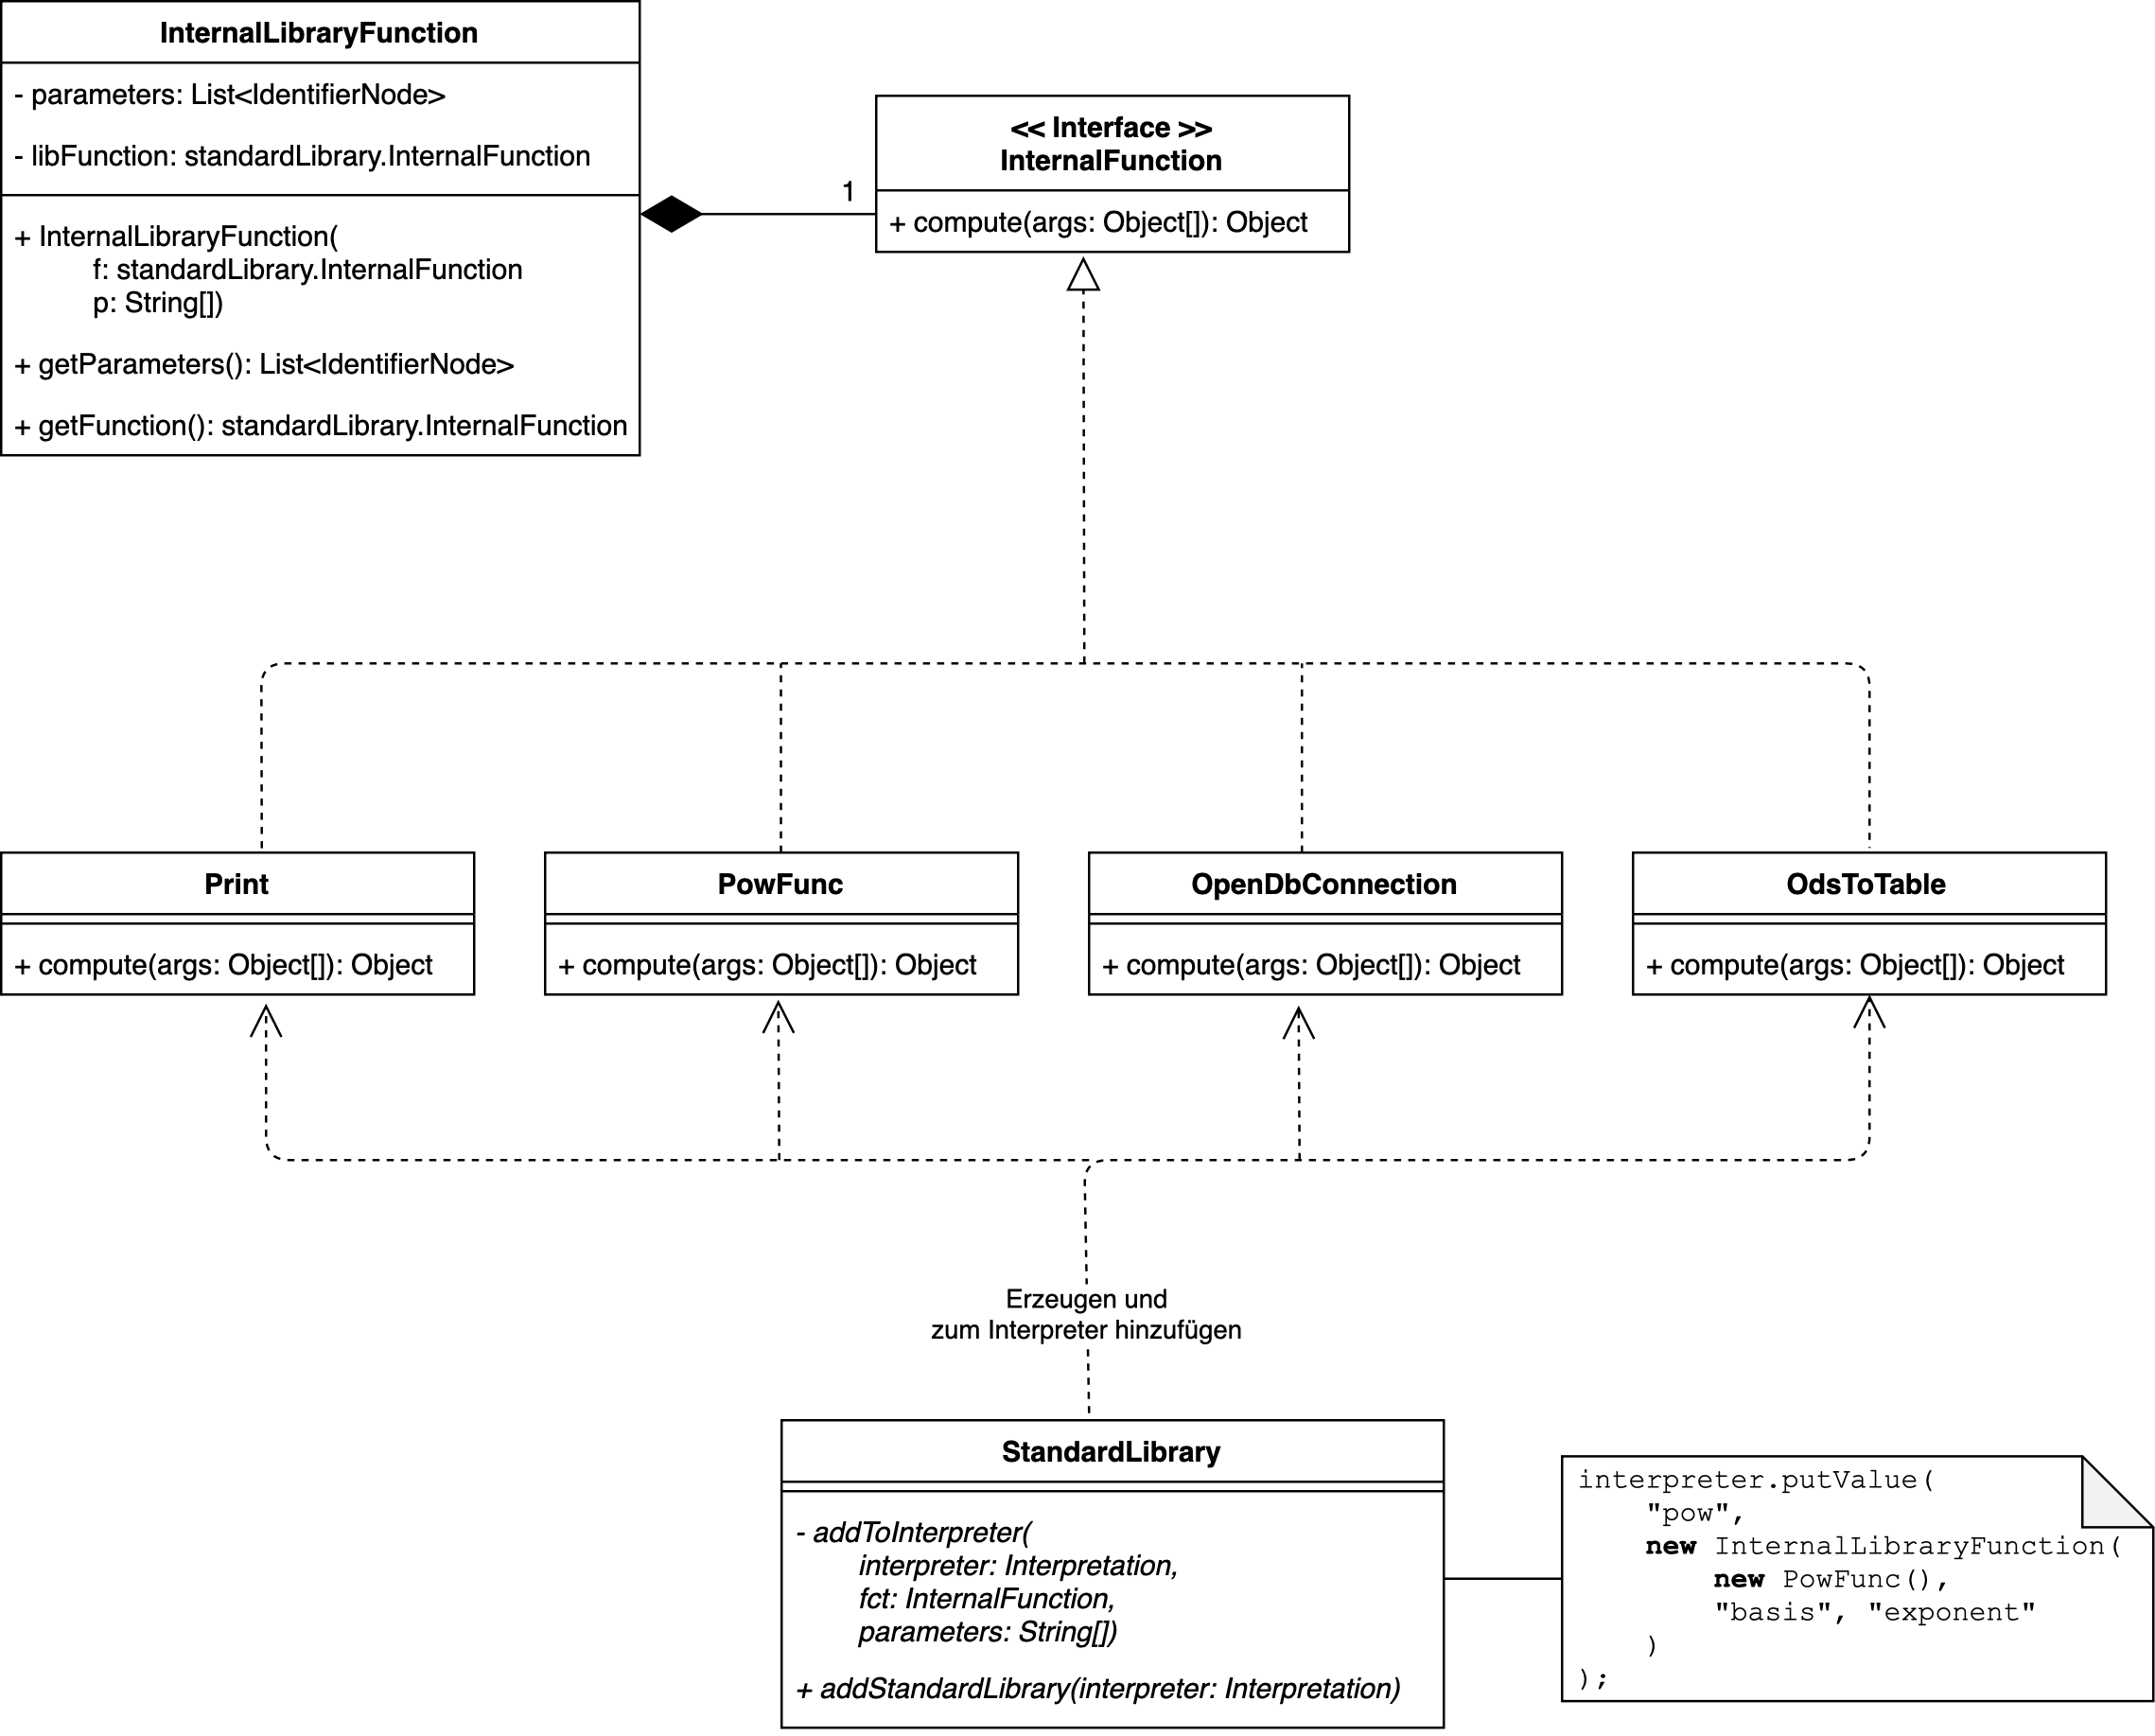
\includegraphics[width=.8\textwidth]{images/standardlib-uml.png}
\caption{Klassendiagramm - Standardbibliothek}
\end{figure}\label{fig:standardlib-uml}

\subsection{VS Code Extension}

Als Proof-of-Concept wurde eine Visual Studio Code Extension erstellt, die die Schlüsselwörter aus Tabulang farblich hervorhebt.
Die dafür benötigten Dateien befinden sich im Ordner \texttt{vscode extension}.

Um von der Extension Gebrauch machen zu können, wird auf die Datei\\
\texttt{vsc-extension-quickstart.md} verwiesen.
Weiterführend kann an der Extension mithilfe der offiziellen Dokumentation von VS Code weitergearbeitet werden: https://code.visualstudio.com/api/language-extensions/overview
